

\documentclass{beamer}

\mode<presentation> {


\usetheme{Madrid}



\setbeamertemplate{footline}[page number] 

\setbeamertemplate{navigation symbols}{} % To remove the navigation symbols from the bottom of all slides uncomment this line
}

\usepackage{graphicx} 


\usepackage{comment}
\usepackage{tikz}
\usepackage{amsmath}
\usepackage{amssymb}
\usepackage{booktabs} 
\usepackage{tikz-cd}
\usepackage{fontawesome}
\usepackage{apacite}
\renewcommand\bibliographytypesize{\footnotesize}
\usepackage{mathtools}
%\usepackage {tikz}
\usepackage{tkz-graph}
\GraphInit[vstyle = Shade]
\tikzset{
  LabelStyle/.style = { rectangle, rounded corners, draw,
                        minimum width = 2em, fill = yellow!50,
                        text = red, font = \bfseries },
  VertexStyle/.append style = { inner sep=5pt,
                                font = \normalsize\bfseries},
  EdgeStyle/.append style = {->, bend left} }
\usetikzlibrary {positioning}
%\usepackage {xcolor}
\definecolor {processblue}{cmyk}{0.96,0,0,0}


\title[Short title]{Progress Report} 

\author{Shakil Rafi} 
\institute[University of Arkansas] 
{
University of Arkansas \\ 
\medskip
}
\date{\today} 

\begin{document}
\nocite{*}
\begin{frame}
\titlepage 
\end{frame}

\begin{frame}
\frametitle{Table of Contents} 
    \tableofcontents 
\end{frame}
\begin{frame}{What to Solve}
    We seek to solve dynamic equilibrium equations. The formulation from Liu and Quek assumes among other things:
    \begin{enumerate}
        \item \textit{Linear Elastic} Deformation grows proportionally with external force.
        \item \textit{Isotropic} Material property is direction independent.
    \end{enumerate}
    We distinguish between four kinds of objects: beams, trusses, plates and shells.
\end{frame}
\begin{frame}{What to Solve}
    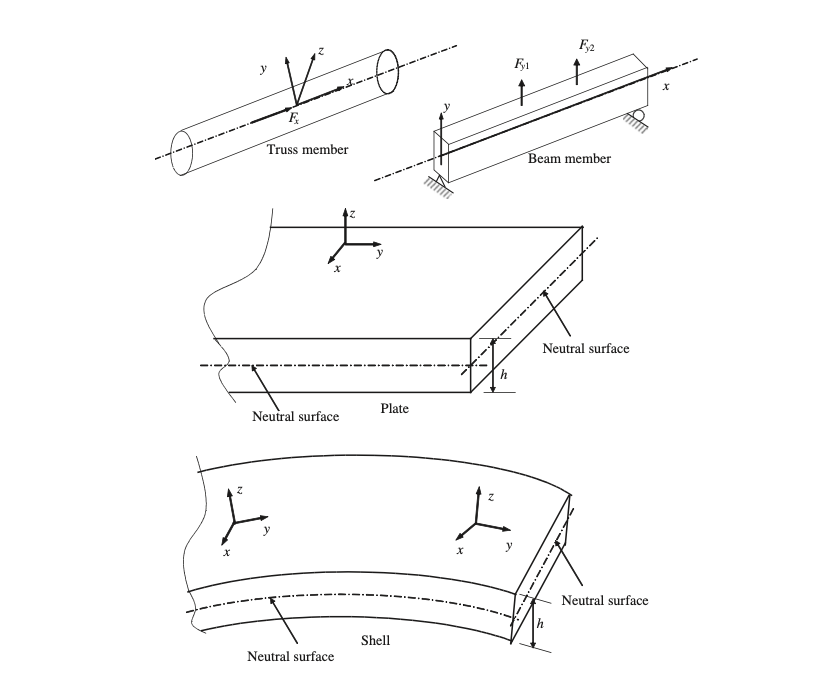
\includegraphics[scale = 0.35]{TypesOfObjects.png}
\end{frame}
\begin{frame}{What to Solve}
    Taking a queue from Liu and Quek, we start off by defining DEE for an idealized infinitesimal, linearly elastic, isotropic material.
    \quad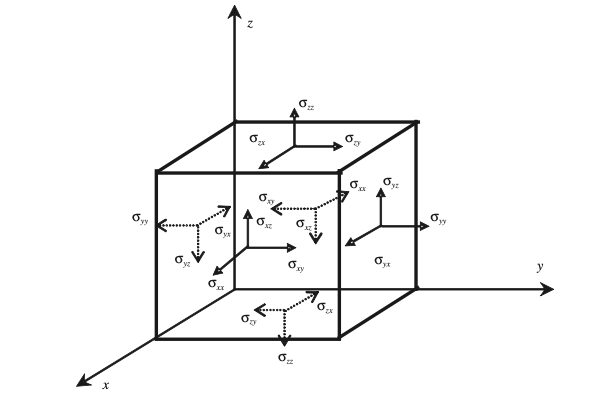
\includegraphics[scale = 0.4]{Cube.png}

    Observe that because of equilibrium $\sigma_{xy} = \sigma_{yx}; \sigma_{xz} = \sigma_{zx}; \sigma_{yz}= \sigma_{yz}$ 
    Which give sus the stress tensors: $\sigma^T = \{\sigma_{xx},\sigma_{yy},\sigma_{zz},\sigma_{yz},\sigma{xz},\sigma{xy}\}$
\end{frame}
\begin{frame}{What to Solve}
    We also get six strain components $\epsilon^T = \{\epsilon_{xx},\epsilon_{yy},\epsilon{zz},\gamma_{yz},\gamma_{xz},\gamma_{xy}$
    Where:
    \begin{align*}
        \epsilon_{xx} &= \frac{\partial u }{\partial x}; \quad \epsilon_{yy} = \frac{\partial v}{\partial y}; \quad \epsilon_{zz} = \frac{\partial w}{\partial z};\\
        \gamma_{xy} &= 2\epsilon_{xy} = \frac{\partial u}{\partial_y} + \frac{\partial v}{\partial x}; \\
        \gamma_{xy} &= 2\epsilon_{xz} = \frac{\partial u}{\partial_z} + \frac{\partial w}{\partial x}; \\
        \gamma_{yz} &= 2\epsilon_{yz} = \frac{\partial v}{\partial_z} + \frac{\partial w}{\partial y}; \\
    \end{align*}
\end{frame}
\begin{frame}{What to Solve}
    Provided $\textbf{U} = \begin{pmatrix}
        u\\
        v\\
        w\\
    \end{pmatrix}$ the displacement matrix we get the system $\epsilon = \textbf{LU}$
    Where the differential operator is:
    $\textbf{L} = \begin{pmatrix}
        \frac{\partial}{\partial x} & 0 & 0\\
        0 & \frac{\partial}{ \partial y} & 0\\
        0 & 0 & \frac{\partial}{\partial z}\\
        0 & \frac{\partial}{\partial z} & \frac{\partial}{\partial y} \\
        \frac{\partial}{\partial z} & 0 & \frac{\partial}{\partial x} \\
        \frac{\partial}{\partial y} & \frac{\partial}{\partial x} & 0 \\
    \end{pmatrix}$

\end{frame}

\end{document}


